% !TEX root=frame_thesis.tex

\addtocontents{toc}{\protect\setcounter{tocdepth}{0}}

\chapter*{Appendix}
\section*{More Details of the Model} \label{sec:APPpopgrowth}
\FloatBarrier
\begin{figure}[h]
	\centering
	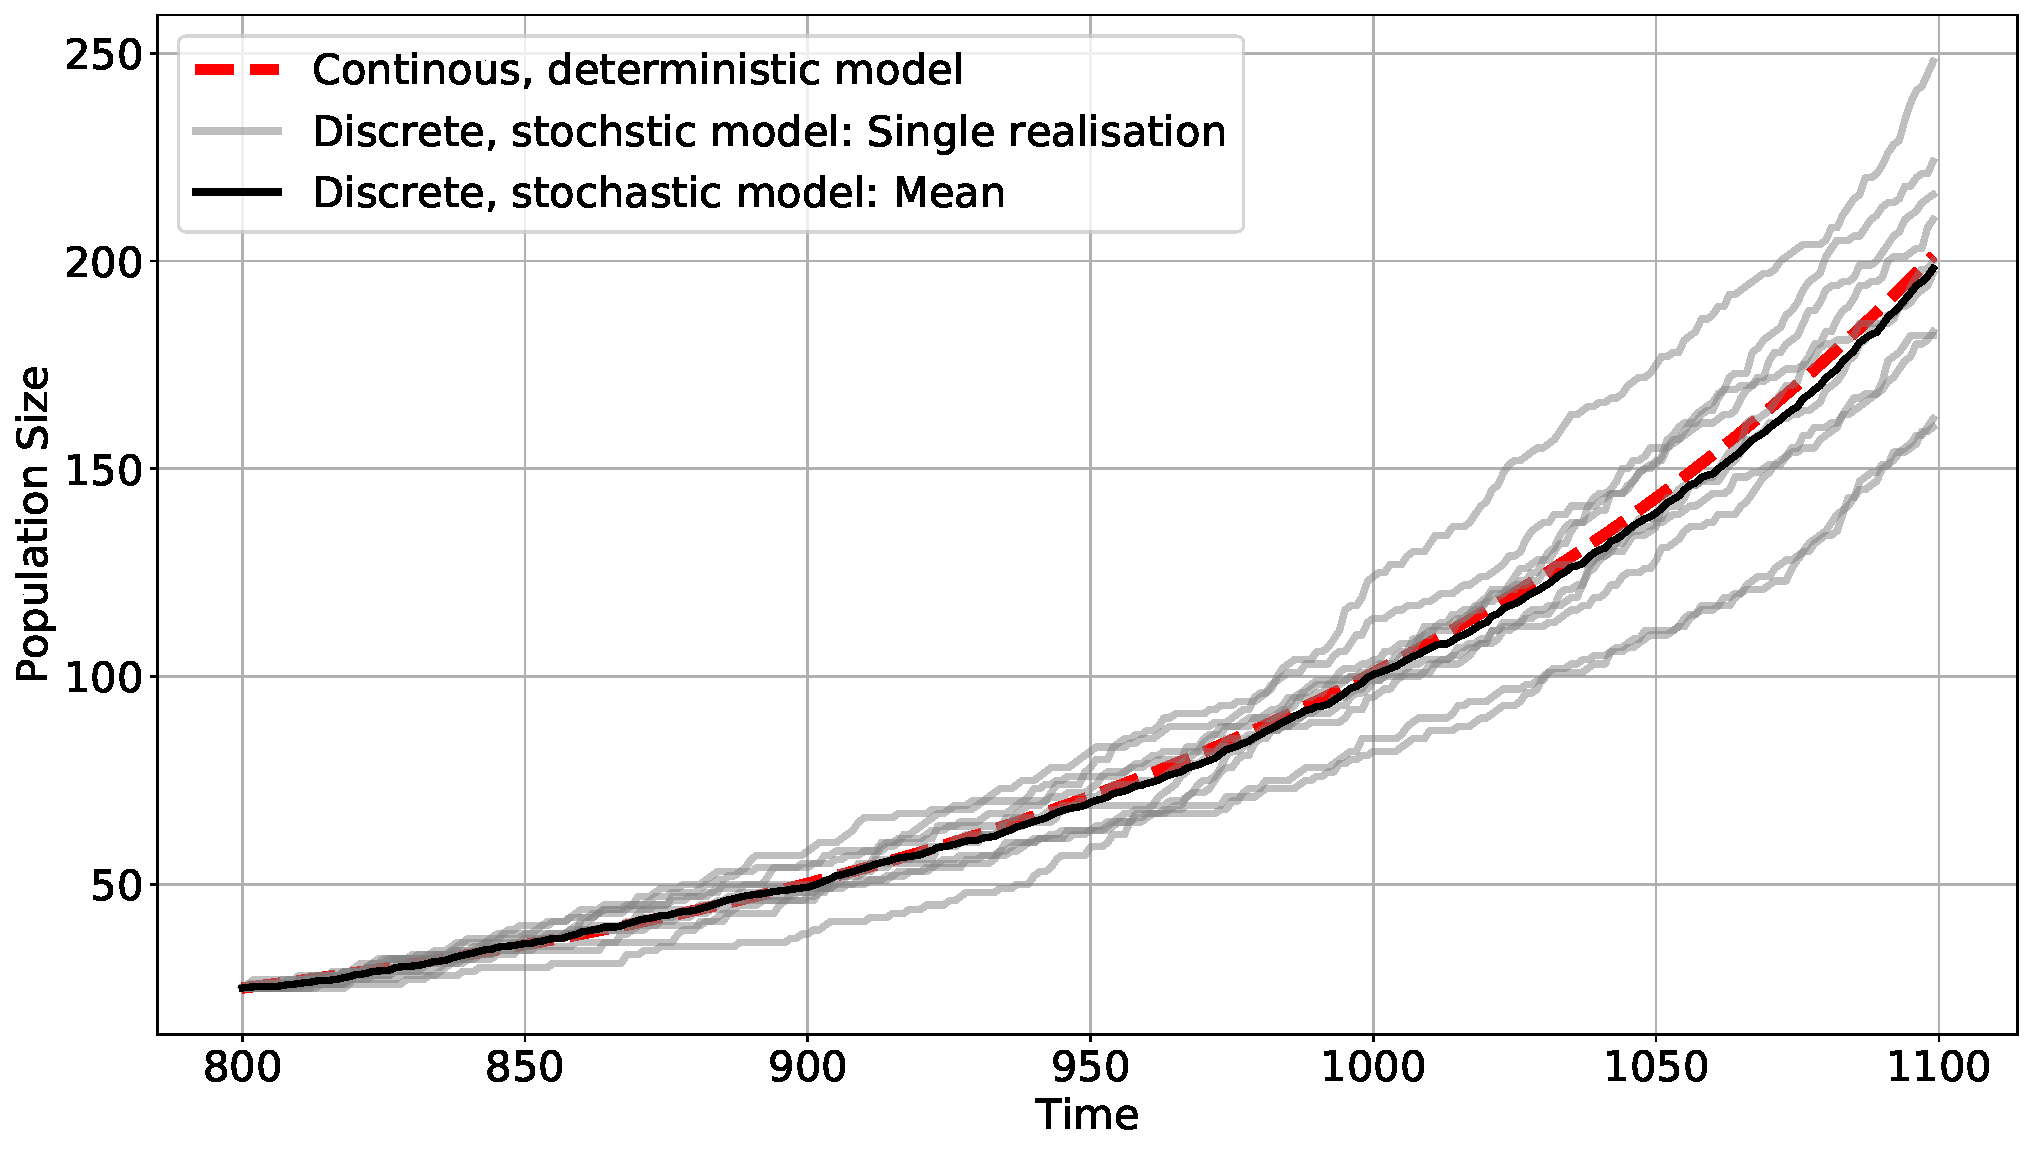
\includegraphics[width=\textwidth]{images/RealisationsOfPopGrowth.pdf}
	\caption{Realisations (and the mean) of the discrete, stochastic population growth model (assuming $H_{\rm i}(t) = 1$ for all $t$ here. In comparison, the continuous exponential growth. The growth rate is $g(H_{\rm i}(t)=1)=1.007$, as in the standard setting of the model.}
	\label{fig:realisationsofpopgrowth}
\end{figure}


\section*{More Results}
\FloatBarrier
\subsection*{Standard Run}
%On \url{https://github.com/PeterSteiglechner/Masterthesis_ZMT_2020}, 
In the supplementary material, I provide an animated figure showing the spatial pattern of Easter Island settlement, deforestation and agricultural production in one single realisation of the standard run over time.

\begin{figure}[h]
	\centering
	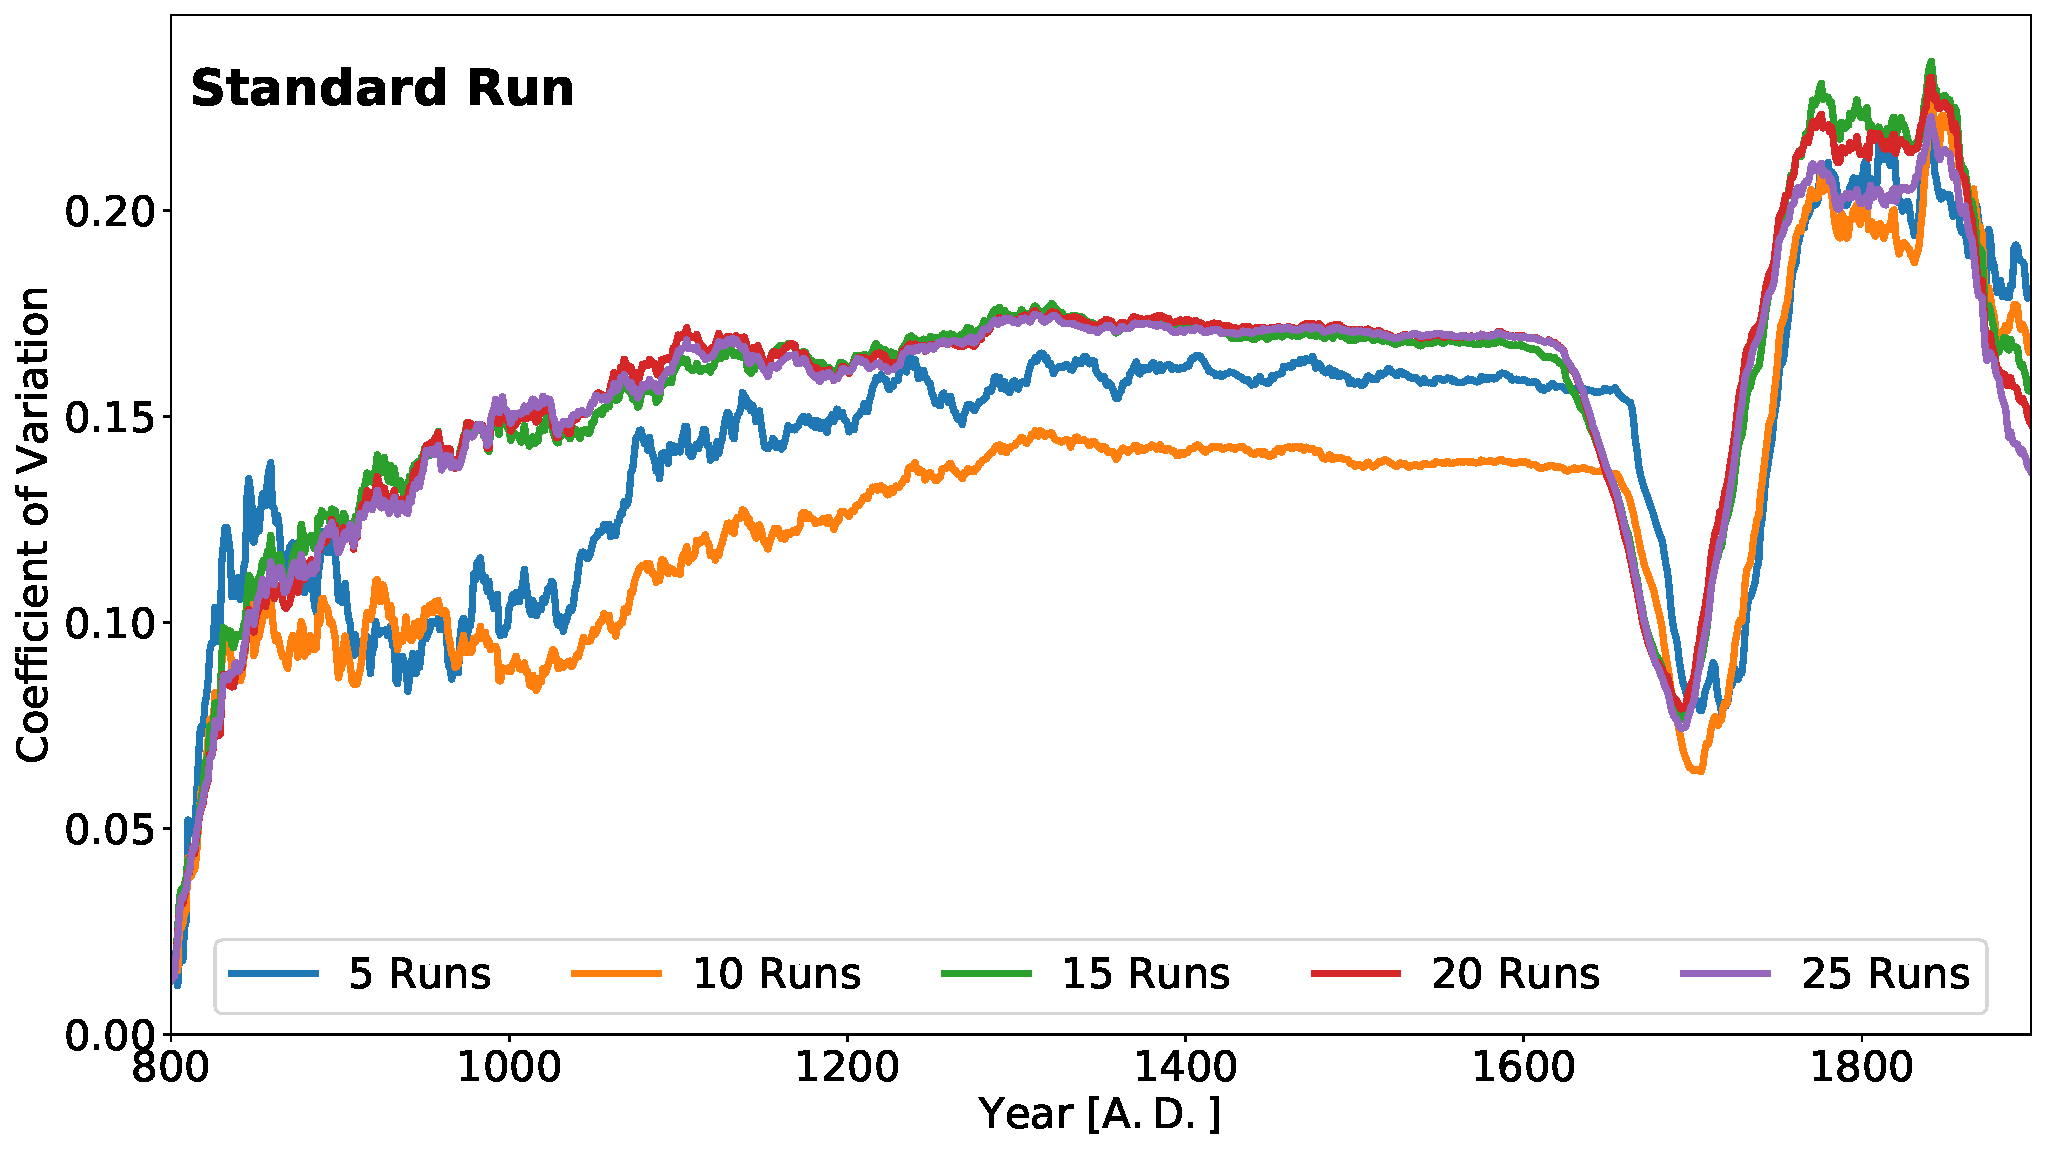
\includegraphics[width=\textwidth]{images/Results/Standard/CoeffOfVariation}
	\caption{The coefficient of variation of ensembles of 5 to 25 runs for the Standard run over time. For more than 15 runs, the coefficient of variation does not change significantly and, thus, this provides a good ensemble size}
	\label{fig:coeffofvariation}
\end{figure}


\begin{figure}[h]
	\centering
	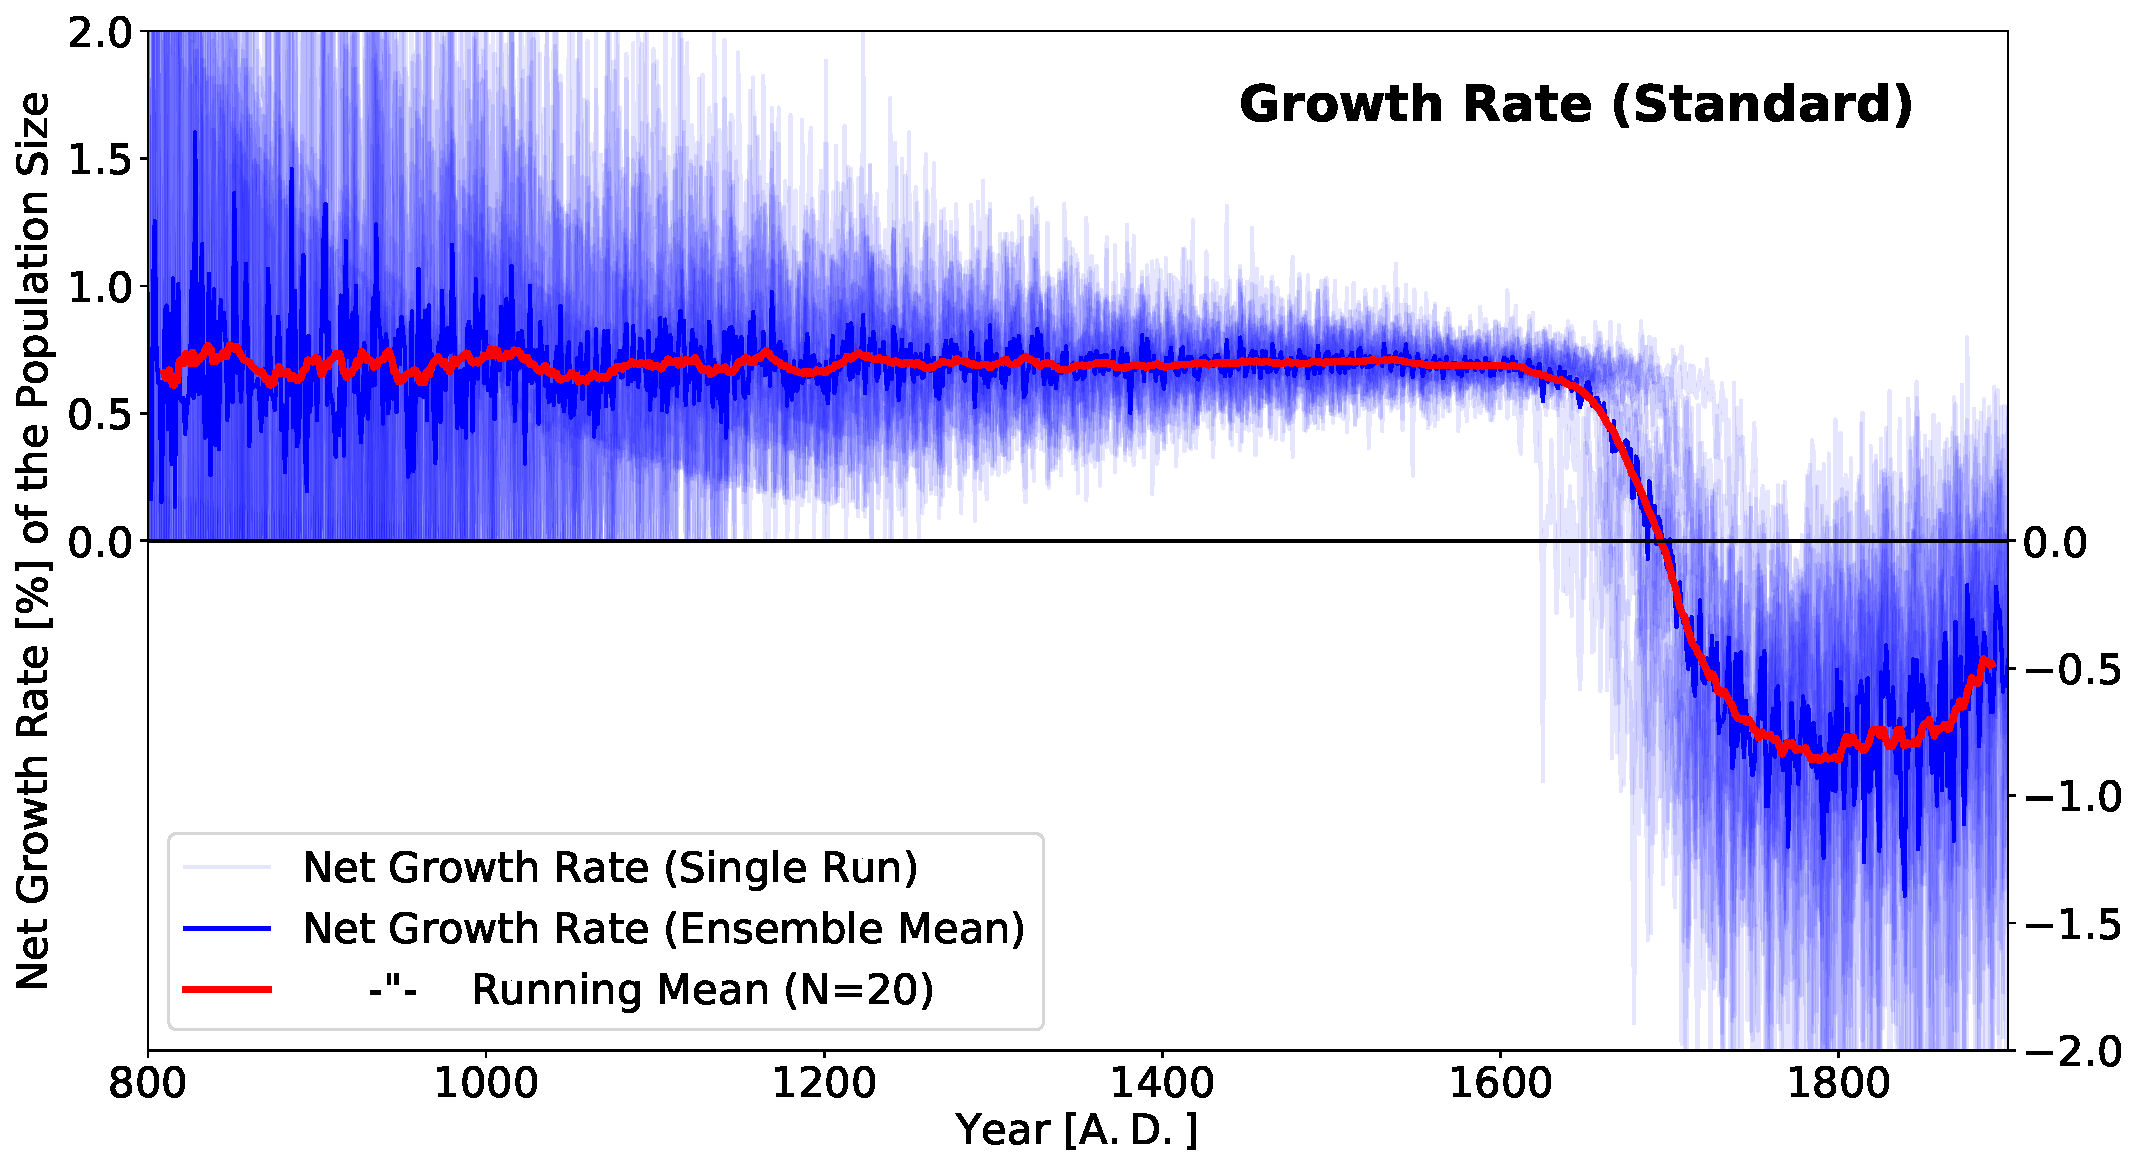
\includegraphics[width=1.0\linewidth]{images/Results/Standard/NetGrowthRate}
	\caption{Ensemble of five Standard runs. The net population growth rate is shown as the mean of the ensemble (blue) and, for easier visibility, as a running mean (red).} 
	\label{fig:app:STDnetgrowthrate}
\end{figure}
\FloatBarrier
\subsection*{Clustering the Agents}
\begin{figure}[h]
	\centering
	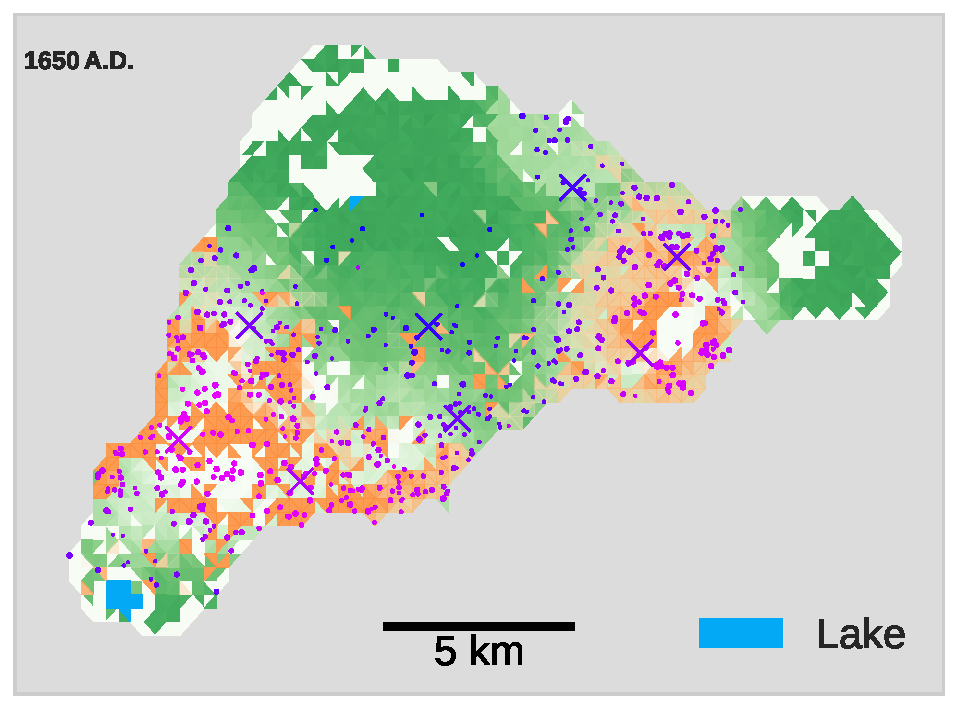
\includegraphics[width=1\linewidth]{images/ClusterSTDS1650}
	\caption{The map shows one realisation of the Standard run. The agents are assigned to clusters with midpoints (crosses) by a k-Means algorithm of the three dimensional state vectors $\left( x_{\rm i}, y_{\rm i}, T_\text{Pref, i} \right)(t)$ for agent $i$ in the year $1650\, {\rm A.D.}$.}
	\label{fig:clusterstds1650}
\end{figure}

\FloatBarrier
\newpage
\subsection*{Variation in the Agents' Adaptation Strategy of the Tree Preference}
\begin{figure}[h]
	\centering
	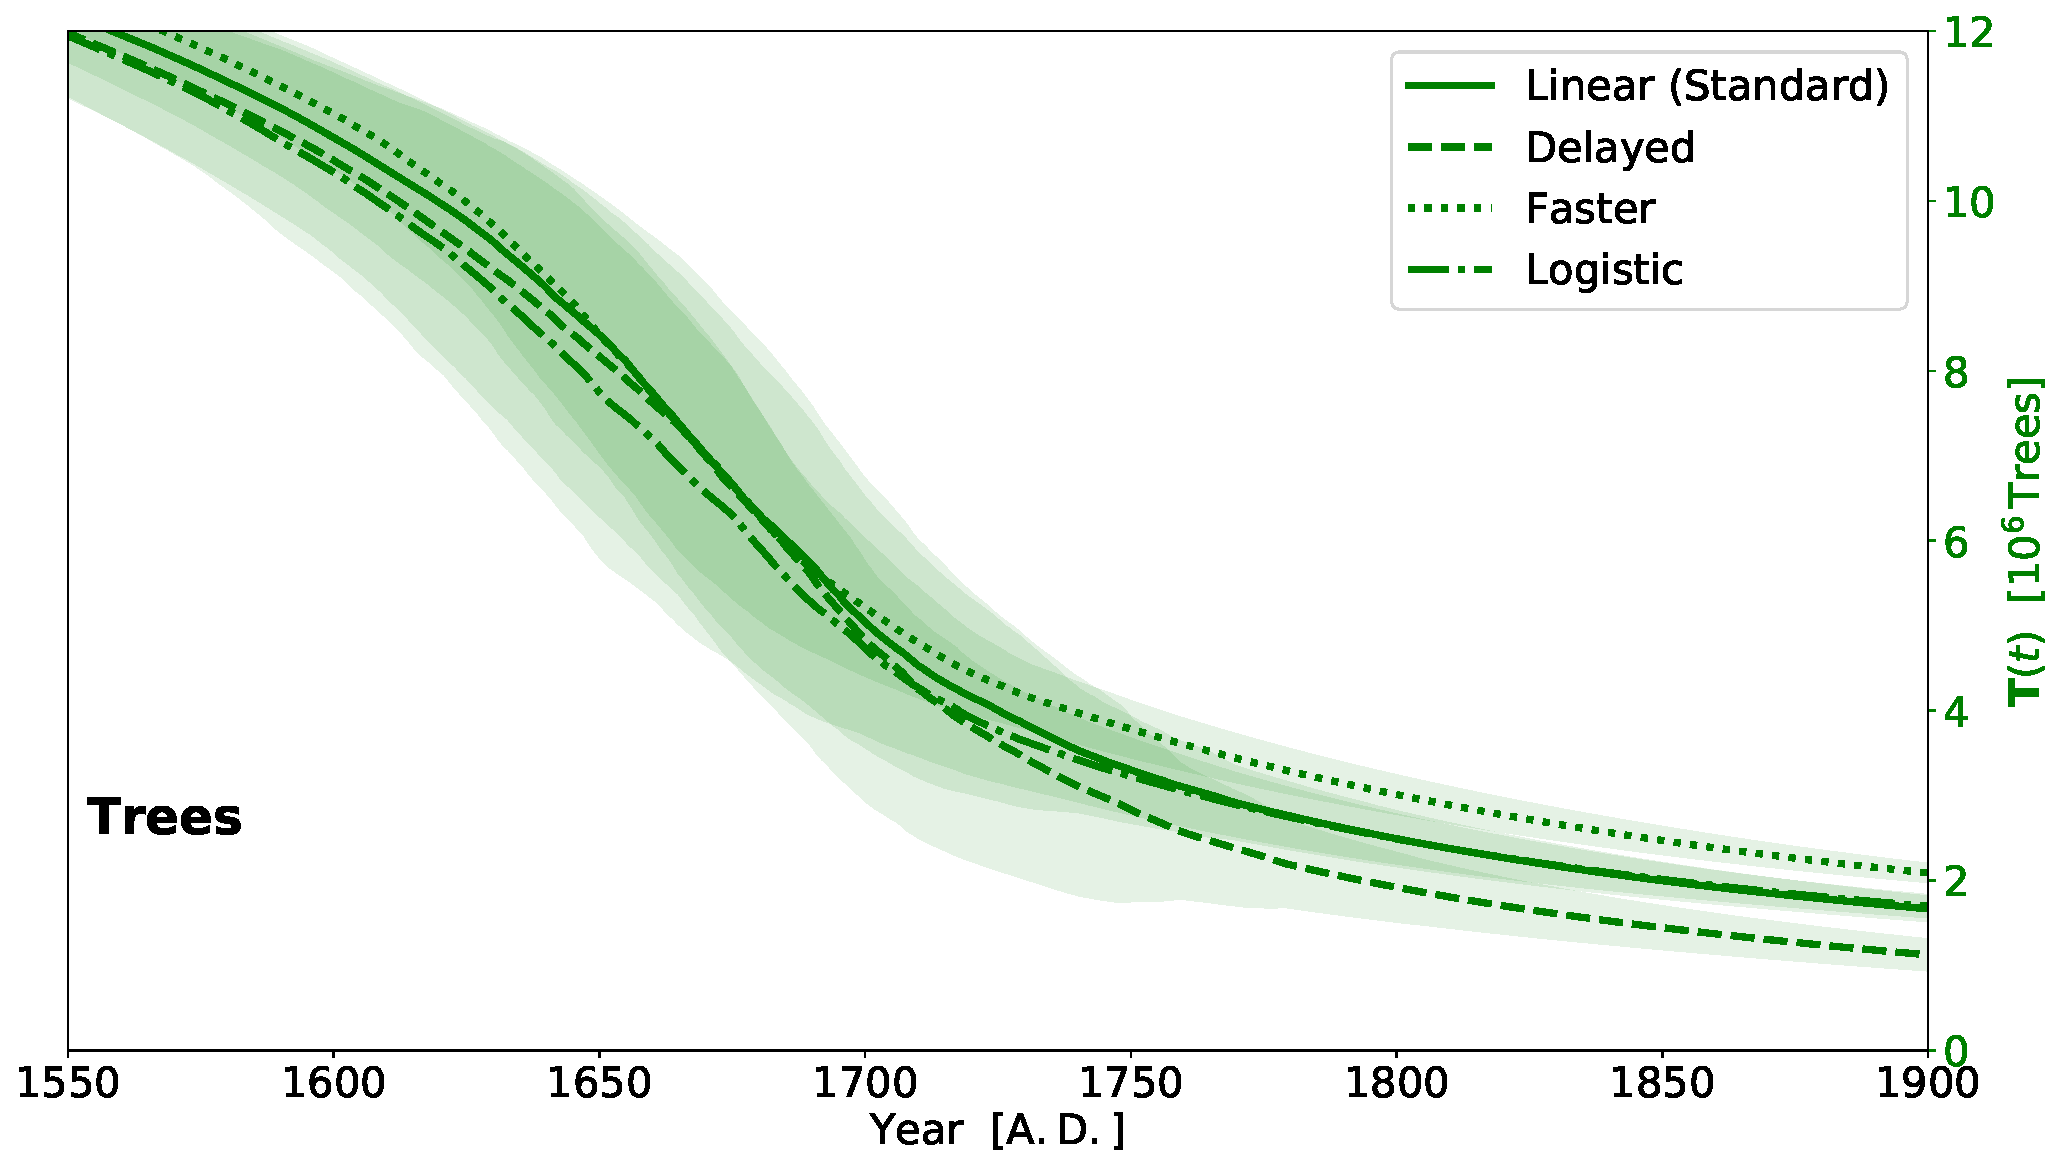
\includegraphics[width=0.9\linewidth]{images/Results/TPref/TPrefAdaption_Trees}
	\caption{Number of Trees for the four different adaptation strategies.}
	\label{fig:tprefadaptiontrees}
\end{figure}
\begin{figure}[h]
	\centering
	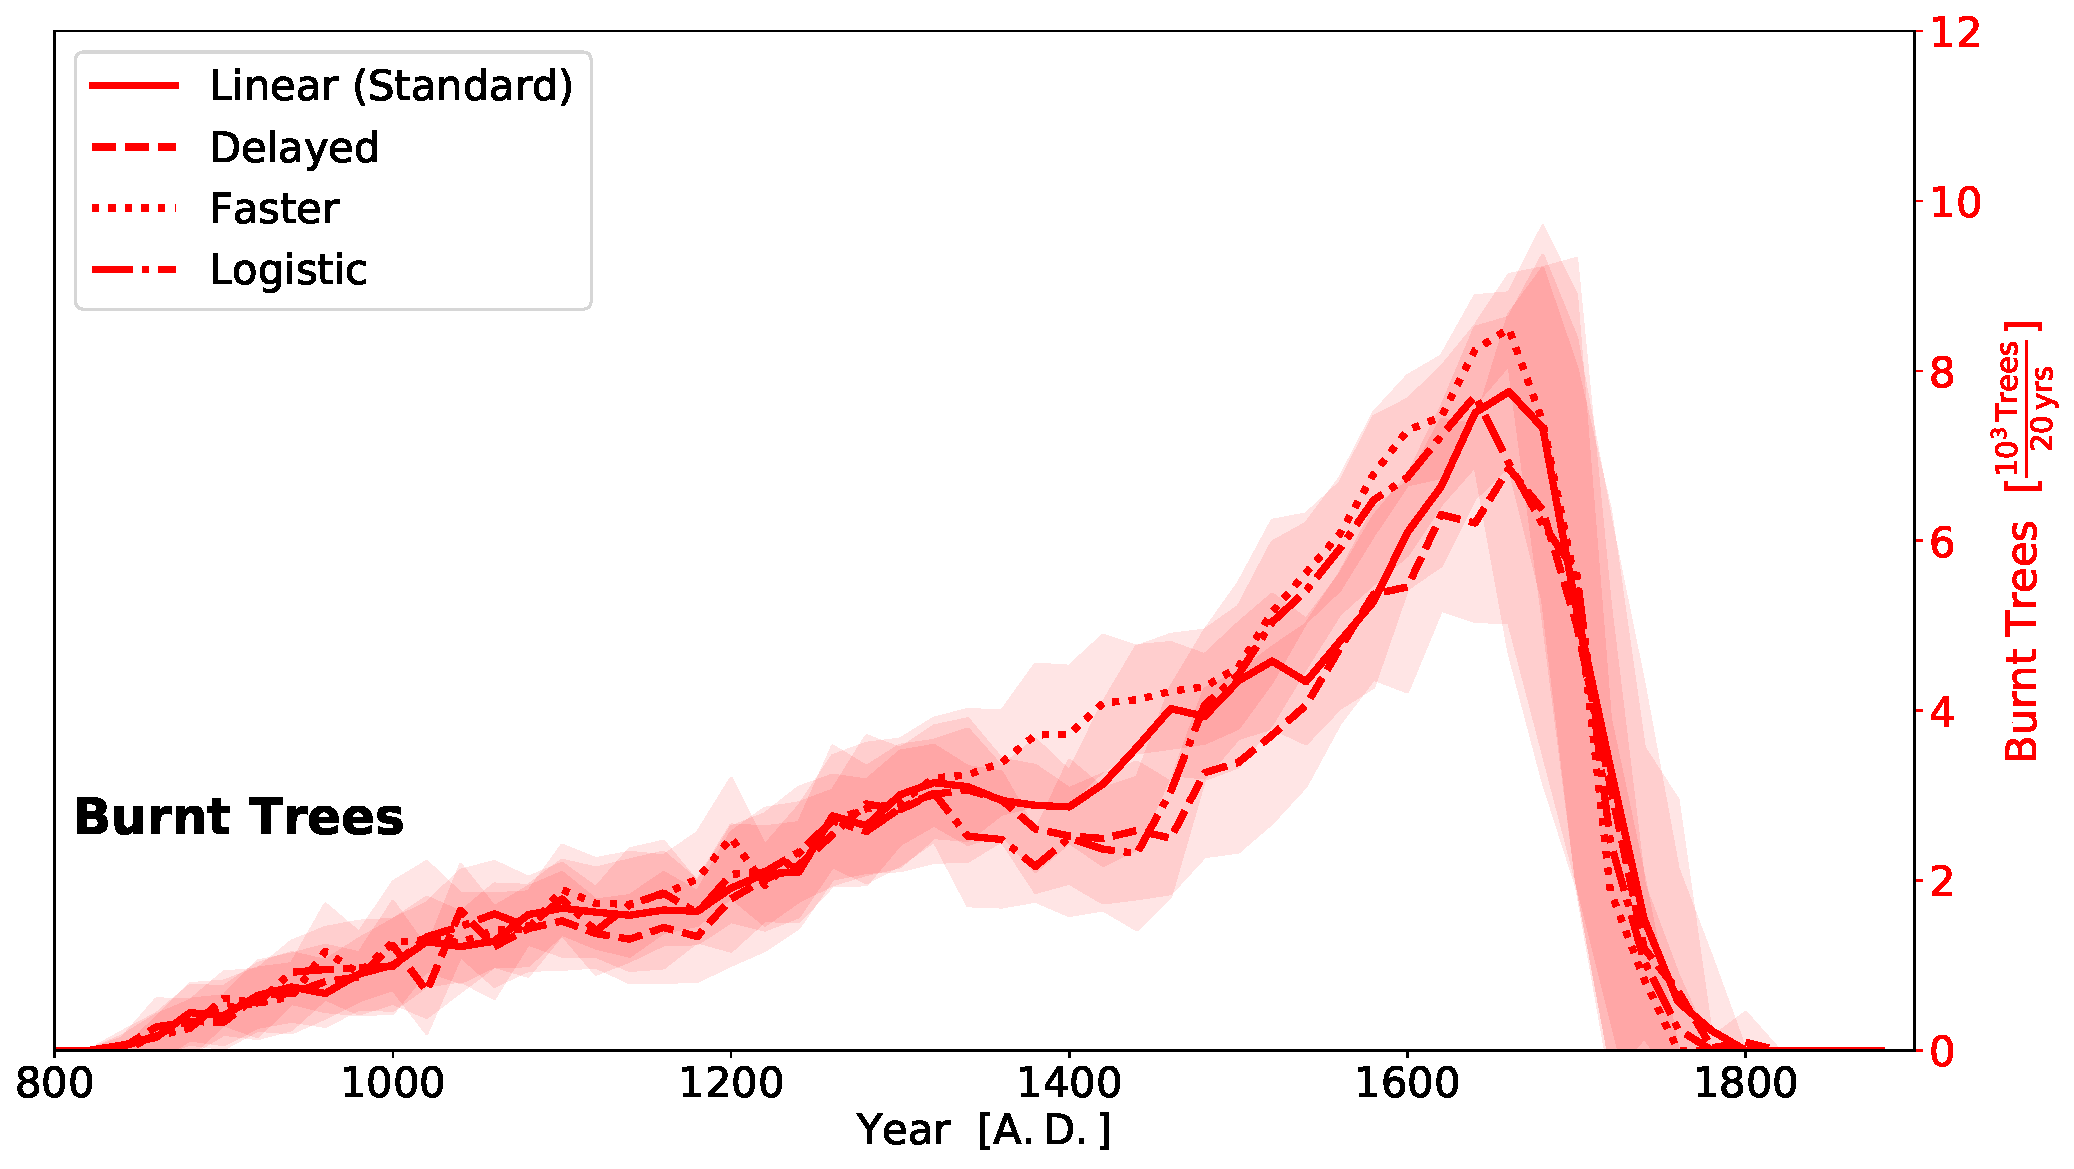
\includegraphics[width=0.90\linewidth]{images/Results/TPref/TPrefAdaption_BurntTrees}
	\caption{Number of Burnt Trees for the four different adaptation strategies.}
	\label{fig:tprefadaptionburnttrees}
\end{figure}